\chapter{Sběr požadavků a analýza}\label{chap:sberpozadavkuaanalyza}

\section{Požadavky}

Následuje seznam funkčních, nefunkčních a vyřazených požadavků na rozšíření aplikace. Funkční a nefunkční požadavky mají pro následnou práci přiřazeny unikátní identifikátory ve tvaru \enquote{F<číslo>}/\enquote{N<číslo>} (kde písmeno značí \textbf{f}unkční/\textbf{n}efunkční požadavek). Hvězdičkou jsou dále označeny požadavky, které vychází z plánovaných rozšíření v rámci bakalářské práce uvedených v sekci~\ref{sec:planrozsirenibp}. Některé plánované změny z této kapitoly byly vyřazeny a je jim věnována poslední podsekce~\ref{subsec:vyrazenepozadavky}.

\subsection{Funkční požadavky}

\begin{enumerate}[label=\textbf{F\arabic*}]
    \item \label{F1} \textbf{evidování zájemců o kurz *:} vzhledem k plnému obsazení všech termínů během týdne je třeba evidovat zájemce o kurzy -- ať už jednotlivce, či zájemce o skupiny -- každý klient může mít zájem o daný kurz nejvýše jednou, je třeba také evidovat k tomuto zájmu text formou poznámky, datum přidání zájemce do evidence a kurz, o který má zájem,
    \item \label{F2} \textbf{kontrola časového konfliktu lekcí *:} současná verze aplikace nijak neřeší časové konflikty lekcí, je třeba zakázat možnost jakéhokoliv překryvu lekcí vzhledem k datu, času a jejich délce, toto se netýká zrušených lekcí, které budou pro řešení konfliktů ignorovány (je třeba zavést~\ref{F19} pro korektní fungování konfliktů),
    \item \label{F3} \textbf{vylepšení předplacených lekcí *:} stávající způsob evidence předplacených lekcí není dostačující -- pro jednotlivce je třeba předplacené lekce přidávat po jednom (klienti si často předplácí více lekcí dopředu), pro skupiny je evidování ještě horší, protože každý člen obvykle platí jinak a na odlišné časové období (případně vždy jen jednu lekci) a prakticky se nedá tato evidence předplacených lekcí ručně udržovat, je to příliš složité,
    \item \label{F4} \textbf{vyhledávání klientů *:} v aplikaci je mnoho klientů a je časově náročně vždy v seznamu vyhledávat příslušného klienta, je třeba zavést možnost vyhledávání v klientech, a to z jakéhokoliv místa aplikace, také je třeba, aby vyhledávání bralo v potaz možné překlepy lektorky v zadávaném výrazu k vyhledávání a také možný překlep ve jménu uloženého klienta, vyhledávalo by se jen mezi aktivními klienty (viz požadavek~\ref{F6}),
    \item \label{F5} \textbf{přepracování formuláře pro lekce:} současný formulář není úplně přehledný, pokud má skupina více než 2 členy, je potřeba neustále posouvat obsahem, protože se nevejde na monitor, je třeba jej kompletně přepracovat dle konzultace s lektorkou, v závislosti na návrhu může souviset s~\ref{F3},
    \item \label{F6} \textbf{zavedení aktivních a neaktivních klientů a skupin:} v evidenci je mnoho klientů a skupin, kteří aktuálně nechodí, ale např. za rok budou opět chodit, je tedy třeba umožnit skrytí všech klientů/skupin, kteří aktuálně na lekce nedochází a k těmto skrytým (neaktivním) klientům/skupinám umožnit přístup, ve výchozím zobrazení ale ukazovat jen aktivní,
    \item \label{F7} \textbf{nastavitelná délka kurzů:} současná verze aplikace automaticky předvyplní dobu trvání lekce v závislosti na tom, zda je skupinová (45~min.) či pro jednotlivce (30~min.) -- to není dostačující, protože např. lekce některých kurzů trvají vždy 45~min. nehledě na počet členů -- je tedy třeba umožnit u kurzu evidovat dobu trvání pro jednotlivce, a tu pak ve výchozím stavu jednotlivcům dávat, pro skupiny stále stačí jedna výchozí hodnota (45~min.),
    \item \label{F8} \textbf{zobrazit poslední transakce na bankovním účtu:} na hlavní stránce je třeba mimo dnešních lekcí třeba zobrazit aktuální zůstatek na bankovním účtu projektu (Fio banka) a transakce za poslední 3~týdny,
    \item \label{F9} \textbf{změny účastníků skupinových lekcí:} někdy se stává, že klient v průběhu kurzu opustí skupinu, v evidenci je již naplánováno několik lekcí dopředu a všech se účastní -- je třeba umožnit při úpravě lekce projevit tyto změny členů skupiny do účastníků dané lekce (v současné době nečlen skupiny zůstává účastníkem lekce a lektorka musí každou lekci ručně smazat a vytvořit znovu bez nečlenů, což je velmi nepohodlné),
    \item \label{F10} \textbf{automatické přidání předplacené lekce:} při omluvě klienta/zrušení ze strany lektorky je třeba automaticky u klienta/skupiny zaznamenat, že mají jeden předplacený termín navíc (v případě, že daný klient měl zaplaceno), v případě jednotlivců je třeba také automaticky zaevidovat, za který den je tato náhradní lekce vytvořena,
    \item \label{F11} \textbf{efektivnější práce v rámci aplikace:} v současné verzi aplikace musela lektorka pro často prováděné činnosti provádět zbytečně mnoho kroků navíc, což činilo příslušné činnosti náročnějšími a snadno se udělala chyba a ztrácel čas -- na základě dalších analýz byly zjištěny problémové oblasti, které vyžadují přepracování: umožnit úpravu lekce (pro jednotlivce i skupiny) z diáře a přehledu, umožnit úpravu klienta/skupiny přímo v kartě klienta/skupiny, umožnit přidání lekce (pro jednotlivce i skupiny) z diáře a přehledu (a to jak s příslušným datem, u kterého bude toto tlačítko, tak i obecně s jakýmkoliv datem), umožnit přidat klienta přímo při přidávání skupiny/zájemce (funkcionalita zájemce implementována v rámci~\ref{F1}),
    \item \label{F12} \textbf{evidování barev kurzů:} je třeba umožnit přiřazení barvy každému kurzu a tuto barvu použít pro rozlišení kurzů napříč celou aplikací, kdekoliv se vyskytuje název kurzu -- lektorka potřebuje okamžitě rozlišit kurzy a mít možnost na první pohled např. v diáři vidět díky barvě, kterého kurzu se barva týká (kurzy mají v rámci propagačních materiálů své ustálené barvy),
    \item \label{F13} \textbf{automatické předvyplnění údajů lekce:} pokud má klient/skupina nějakou historii v evidenci, při přidávání nové lekce je třeba na základě této historie předvyplnit vhodnými hodnotami datum, čas a kurz nové lekce -- je tedy třeba vhodně zvolit lekci klienta z jeho historie, podle které budou tyto údaje vypočteny  -- smyslem je těmito výchozími hodnotami vystihnout co nejvíce případu tak, aby lektorka musela tyto hodnoty co nejméně často upravovat,
    \item \label{F14} \textbf{upozornění na ztrátu dat formulářů:} při vyplňování formulářů lektorka občas omylem formulář zavře a přijde o úpravy, je třeba zavést ochranu, která tomuto zabrání (a zároveň ale nebude zbytečně upozorňovat na ztrátu dat, když k žádné změně nedošlo),
    \item \label{F15} \textbf{vylepšení chybových hlášení:} chybová hlášení jsou někdy málo podrobná, případně nezmiňují možnosti řešení, zobrazují se krátce, případně dojde k neošetřené chybě na serveru a klientská část pak nedokáže korektně uživateli popsat, kde je problém,
    \item \label{F16} \textbf{titulky stránek:} každá stránka by měla mít v prohlížeči svůj titulek, v současné době má každá stránka stejný titulek a lektorka tak nemá možnost jednoduše rozlišit, který panel má otevřenou kterou stránku aplikace,
    \item \label{F17} \textbf{nastavitelné vlastnosti stavů účasti:} některé stavy účasti mají pro některé výpočty v rámci aplikace speciální význam (např. omluvené lekce se nezapočítávají do počtu absolvovaných lekcí klienta, další stav znamená, že klient dorazí a tento stav je zároveň výchozí), toto svázání stavu účasti s významem je ale založeno na názvu stavu účasti (a pevně nadefinováno v kódu), lektorka si chce ale název příslušných stavů účasti sama měnit a je třeba pro to zavést příslušné možnosti,
    \item \label{F18} \textbf{omezení a validace hodnot:} je třeba provést revizi stávajících omezení na jednotlivé hodnoty v rámci aplikace (API a databáze) i klientské části, zavést nová omezení pro nové funkční požadavky a zdokumentovat všechna aktuální omezení a validace prováděná nad celou doménou,
    \item \label{F19} \textbf{automatické zrušení lekce:} pokud nikdo z účastníků nemá dorazit (všichni jsou omluveni), lekce má být automaticky zrušena,
    \item \label{F20} \textbf{zobrazení zrušených lekcí:} v přehledu na hlavní stránce a v diáři je třeba zobrazit i zrušené lekce, v současné verzi se nezobrazují (to byl původní požadavek, ale nakonec se ukázal jako nesprávný a lektorka lekce potřebuje vidět nejen v kartě klienta),
    \item \label{F21} \textbf{skupinové lekce bez účastníků:} lektorka potřebuje vytvářet lekce pro skupiny bez účastníků (plánuje dopředu termíny a členy přidá až když budou známí) -- současná aplikace na toto nebyla připravena, klientská část aplikace dokonce při přidání takové lekce spadne.
\end{enumerate}

\subsection{Nefunkční požadavky}

\begin{enumerate}[label=\textbf{N\arabic*}]
    \item \label{N1} \textbf{dokumentace:} dokumentace v kódu pro serverovou i klientskou část, dokumentace API,
    \item \label{N2} \textbf{testování *:} aplikace prakticky neobsahuje žádné testy (jen několik základních \enquote{smoke} testů), je třeba zavést API a UI (e2e) testy pro klíčové části aplikace a průchody v aplikaci,
    \item \label{N3} \textbf{zavedení nástrojů pro usnadnění vývoje a údržby:} je třeba zavést nástroje pro monitorování chyb v aplikaci, správu logů (vyhledávání, ukládání), statické typování a analýzu kódu -- k tomu byla provedena v teoretické části rešerše v kapitole~\ref{chap:nastrojeprousnadnenivyvojeaudrzby},
    \item \label{N4} \textbf{revize bezpečnosti:} je třeba provést kompletní revizi aplikace z hlediska bezpečnosti a opravit případné slabiny, problémy či zranitelnosti, provést aktualizace závislostí apod.,
    \item \label{N5} \textbf{vylepšení použitelnosti:} z hlášení lektorky a také z vlastní analýzy vyplývá, že je třeba se zaměřit na opravení problémů s použitelností a její vylepšení,
    \item \label{N6} \textbf{rychlejší získání dat z API *:} pokud klientská část má někde zobrazit více dat, požadavek někdy probíhá enormně dlouho a dokonce může být ze strany Heroku pro dlouhou prodlevu zastaven a lektorka si data nezobrazí -- je třeba nalézt úzké hrdlo aplikace, které toto zpomalení v jednotkách případů (když je hodně dat) zpomaluje a toto vylepšit, také je třeba se zaměřit na optimalizaci počtu požadavků na API (zda některé nelze uložit a znovupoužít bez dalšího provádění, viz možné rozšíření o React Context API v sekci~\ref{sec:planrozsirenibp}) a případně zjednodušení obsahu odpovědí díky znovupoužívání,
    \item \label{N7} \textbf{konfigurace více prostředí:} pokud se aplikace úspěšně sestaví na integračním serveru, nahraje se na produkci \cite{bp} -- to může v případě neodhalené chyby v aplikaci způsobit okamžitý pád produkce a případně i ztrátu dat -- toto souvisí s lepším pokrytím testy (viz \ref{N2}), ale je třeba také zavést další prostředí, do kterých se v různé fázi bude aplikace nasazovat, a to tak, aby bylo k dispozici jak prostředí naprosto totožné s produkcí (např. pro reprodukování chyb hlášených koncovým uživatelem), tak prostředí opět postavené na tom produkčním, ale s novější nasazenou verzí aplikace -- kompletní návrh bude popsán v sekci~\ref{sec:konfiguraceviceprostredi},
    \item \label{N8} \textbf{zálohy databáze:} je třeba zavést pravidelné automatické zálohování databáze z produkce.
\end{enumerate}

\subsection{Vyřazené požadavky}\label{subsec:vyrazenepozadavky}
\begin{itemize}
    \item \textbf{evidence pomůcek a učebnic *:} v rámci projektu ÚP již existuje starší aplikace na míru, která tuto funkcionalitu dostatečně řeší a zatím není potřeba toto řešení integrovat do jednotného řešení,
    \item \textbf{offline přístup a SSR *:} co se týče SSR, načítání aplikace je dostatečně rychlé a není zde tedy potřeba prozatím SSR řešit, řešení offline režimu zatím není ze strany lektorky požadováno (stačí jí stávající řešení).
\end{itemize}

\section{Detailní analýza některých požadavků}

Některé požadavky nejsou úplně přesně definované a před dalším pokračováním je třeba je dodefinovat.

\subsection{F3 - vylepšení předplacených lekcí}

Detailní analýza požadavku~\ref{F3}.
V případě jednotlivců je problém s tím, že je předplacené lekce přidávat po jednom -- zde bude lektorce vyhovovat ve formuláři pro přidání lekce možnost uvést počet přidávaných předplacených lekcí, tedy bude zakomponováno v rámci \ref{F5}.

Předplacené lekce skupin jsou evidovány v současné verzi stejným způsobem, tedy lekce je označena jako předplacená, jen je možné zvolit, kteří ze členů skupiny ji skutečně mají předplacenou -- už zde začíná první problém, kdy lekce je předplacená, ale někteří klienti si ji nepředplatili, což je sice korektně zaznamenáno, ale situace začíná být nepřehledná. Při dalších předplacených lekcích, zejména když si jeden účastník zaplatí celou lekci dopředu pak všichni ostatní evidovanou platbu nemají a platí v jiném časovém horizontu, tato situace je už velmi nepřehledná a může vyústit v chyby lektorky kvůli nepřehlednosti. Zde by lektorce vyhovovaly počítadla předplacených lekcí každého klienta, což vyřeší všechny zmíněné problémy. Z počítadel by se při přidávání nové lekce automaticky odečítalo.

Řešení pomocí počítadel vypadá jako ideální řešení i pro jednotlivce, zde by ale byl problém s faktem, že mohou chodit na více kurzů, tedy nelze mít centrální počítadlo pro všechny (na některé kurzy už nechodí, předplácí třeba jen některé, na které chodí apod.), bylo by třeba mít pro každý kurz počítadlo zvlášť, ale v tom případě by pak už nebylo možné evidovat v rámci \ref{F10}, za který den daná předplacená lekce tvoří náhradu (resp. možné by to bylo, ale značně by to zkomplikovalo jak implementaci, tak i práci lektorky), proto je řešení předplacených lekcí pro jednotlivce a skupiny odlišné.

\subsection{F13 -- automatické předvyplnění údajů lekce}

Detailní analýza požadavku~\ref{F13}.
Smyslem tohoto požadavku je předvyplnit datum, čas a kurz nově přidávané lekce podle minulých lekcí, a to tak, aby muselo být do těchto hodnot co nejméně ze strany lektorky zasahováno. Lekce se nejčastěji konají jednou za týden a obvykle ve stejný čas a patří samozřejmě k téže kurzu. Stačí tedy vhodně zvolit referenční lekci a z ní tyto údaje odvodit. V závislosti na podobě historie klienta/skupiny je třeba pokrýt možné případy výběru lekce.

Případy výběru lekce:
\begin{enumerate}
    \item V případě, že klient na žádné lekci ještě nebyl, neodvodíme nic a údaje zůstanou nepředvyplněné.
    
    V případě skupiny bez lekcí datum a čas také v tomto případě neodvodíme, kurz je ale jasný z atributů skupiny.
    \item V případě, že klient chodí na jeden jediný kurz, vyber tento kurz a datum a čas zvol o týden později oproti poslední lekci tohoto kurzu (poslední lekce může být jen předplacená, tedy z té odvoď pouze kurz).
    
    Pro skupiny platí totéž, jen datum a čas bude odvozen vždy, protože předplacené lekce budou v rámci F3 evidovány jinak než u jednotlivců.
    \item V případě, že klient chodí/chodil na více kurzů, vyber ten kurz, jehož poslední lekce je nejpozději (a z té odvoď všechny údaje), navíc, pokud některý kurz má předplacené lekce, preferuj ten (a tedy odvoď jen kurz).
    
    Skupina v této situaci být nemůže, protože má vždy jen lekce k jednomu kurzu.
\end{enumerate}

\subsection{F18 -- omezení a validace hodnot}

Detailní analýza požadavku~\ref{F18}.
V rámci tohoto požadavku bylo třeba vytvořit kompletní seznam všech omezení a validací, které v aplikaci mají být, a to i s ohledem na všechny nové funkční požadavky. Všechna tato omezení byla v rámci analýzy definována. Jejich seznam a rozdělení je vidět v obrázku~\ref{fig:db-model} s návrhem aktualizovaného logického datového modelu.

\subsection{N4 -- revize bezpečnosti}\label{subsec:N4detail}

Detailní analýza požadavku~\ref{N4}.
V rámci tohoto požadavku je potřeba zjistit problémové oblasti a případně i konkrétní problémy, na které se zaměřit. Bylo tedy třeba projít např. konfiguraci aplikace, testovat chování aplikace a také použít nástroj \href{https://observatory.mozilla.org/}{Mozilla Observatory}, který skenuje webové stránky a kontroluje jejich zabezpečení \cite{mozillaobservatory}. Bylo zjištěno několik problémů níže, mají opět unikátní identifikátor, kde písmeno \enquote{B} značí problém s \textbf{b}ezpečností.

Nalezené problémy:
\begin{enumerate}[label=\textbf{B\arabic*}]
    \item \label{B1} \textbf{aktualizace závislostí:} je třeba aktualizovat všechny závislosti (používané knihovny a nástroje) kvůli opravám chyb, zranitelností, ale i novým funkcím -- např. knihovny klientské části při použití příkazu \verb|yarn audit| (pro který musela být i upravena verze yarn, protože v požadované verzi v rámci projektu tento příkaz ani není) bylo nalezeno 36 zranitelností, také je třeba zohlednit u knihoven sémantické verzování a povolit zpětně kompatibilní aktualizace,
    \item \label{B2} \textbf{sjednocení konfigurací:} v rámci produkční konfigurace je možné některá nastavení sloučit s konfigurací lokální verze -- kromě zvýšení bezpečnosti dojde především také ke zvýšení konzistence mezi těmito verzemi aplikace a tedy v budoucnu méně problémy kvůli odlišnostem,
    \item \label{B3} \textbf{deaktivace DEBUG módu:} produkční konfigurace pro 
    Django obsahuje nastavenou proměnnou \verb|DEBUG = True|, na produkci toto nastavení ale být nesmí -- jedná se jak o bezpečnostní (náhled útočníka do metadat aplikace, některých proměnných prostředí ad.), tak výkonnostní problém (zbytečné režijní náklady a vysoké nároky na paměť kvůli ukládání všech SQL dotazů) -- na produkci je tedy třeba nastavit \verb|DEBUG = False| \cite{django-debug},
    \item \label{B4} \textbf{HTTP hlavičky:} díky nástroji Mozilla Observatory bylo zjištěno, že v aplikaci chybí nastavení některých HTTP (Hypertext Transfer Protocol) hlaviček -- Referrer Policy, CSP (Content Security Policy), HSTS (HTTP Strict Transport Security) -- podrobnému popisu významu se budu věnovat v TODO,
    \item \label{B5} \textbf{sjednocení práce s tokeny:} je třeba sjednotit práci s citlivými tokeny a dalšími podobnými elementy -- těchto citlivých dat bude vzhledem k požadavkům přibývat (např. přístup do banky) a je třeba zavést centrální místo správy, kterým budou proměnné prostředí (nyní jsou některé tokeny zašifrované např. v rámci souboru s konfigurací Travisu, některé kvůli své povaze zašifrované nejsou apod.), nebude tak hrozit žádný únik např. ve verzovacím systému (který již nastal i v případě tohoto projektu, kdy kvůli bezpečnostnímu problému s FontAwesome PRO \cite{fontawesome-token} došlo k úniku tokenu pro přístup k placeným ikonám prostřednictvím souboru \verb|yarn.lock|, což by znamenalo problém právě při zveřejnění repozitáře, což je jeden z úkolů této práce), zavedení proměnných prostředí umožní také jednoduchou práci s více prostředími (viz \ref{N7}),
    \item \label{B6} \textbf{zákaz robotů:} roboti mohou přistupovat na stránku s aplikací (např. indexovací robot Google) -- přístup robotům je třeba zakázat, indexace není potřeba a jediným výsledkem je zbytečná spotřeba výpočetního výkonu.
\end{enumerate}


\subsection{N5 -- vylepšení použitelnosti}

Detailní analýza požadavku~\ref{N5}.
Pro zjištění problémů v oblasti použitelnosti a přístupnosti bylo zvoleno několik metod -- Nielsenova heuristická analýza, WCAG~2.1 (Web Content Accessibility Guidelines) a uživatelské testování použitelnosti formou pozorování lektorky při každodenní práci v aplikaci. 

Nielsenova heuristická analýza obsahuje 10~základních pravidel použitelnosti \cite{nielson}: viditelnost stavu systému, spojení mezi systémem a reálným světem, uživatelská kontrola a svoboda, konzistence a standardizace, prevence chyb, rozpoznání místo vzpomínání, flexibilní a efektivní použití, estetický a minimalistický design, pomoc uživatelům poznat, pochopit a vzpamatovat se z chyb, nápověda a návody. Tyto body jsou v rámci této heuristiky dále detailněji popsány \cite{nielson}.

Doporučení WCAG~2.1 vytvořené v rámci konsorcia W3C (World Wide Web Consortium) je v současnosti nejrozšířenější a celosvětově uznávaná metodika tvorby přístupného webového obsahu \cite{wcag-zdrojak}. Následování těchto doporučení učiní obsah přístupnější pro větší okruh uživatelů s různým zdravotním postižením \cite{wcag}. Díky aplikaci doporučení je často webový obsah také více použitelný obecně pro všechny uživatele \cite{wcag} -- a toto je důvod, proč se na tato doporučení zaměřuji v rámci vylepšení použitelnosti aktuální aplikace. Smyslem tedy bude na základě doporučení ověřit a případně napravit problémy s použitelností, které může pocítit i sama lektorka.

Některé zjištěné problémy jsou již v požadavcích definovány, jiné jsou úplně nové. Podle toho problémy rozdělím a navíc ty nové opět opatřím unikátním identifikátorem, kde písmeno \enquote{P} značí problém s \textbf{p}oužitelností.

Seznam nových zjištěných problémů:
\begin{enumerate}[label=\textbf{P\arabic*}]
    \item \label{P1} \textbf{délka načítání:} při delším načítání není uživatel nijak informován, že je vše v pořádku a aplikace stále pracuje -- je třeba při delším načítání uživatele upozornit, že je vše v pořádku a v případě, že načítání trvá přespříliš dlouho, nabídnout mu nějaké řešení,
    \item \label{P2} \textbf{popis netextových prvků:} některé netextové prvky úplně postrádají popis (např. po najetí myší), případně jej obsahují, ale formou \verb|title|, tedy nelze zobrazit na mobilních zařízeních -- je třeba popisy zavést všude a umožnit zobrazení i na mobilních zařízeních,
    \item \label{P3} \textbf{favicon:} v záložce prohlížeče není ikona (favicon) -- dodat,
    \item \label{P4} \textbf{posouvání modálního okna:} v modálním okně se na iOS nedá plynule posouvat -- opravit,
    \item \label{P5} \textbf{react-select:} některé prvky pro výběr (\verb|select|) jsou řešeny uživatelsky přívětivým \verb|react-select| (výběr členů skupiny), některé (výběr kurzu) ale ne a nedá se v nich tak např. vyhledávat či jednotlivé položky odlišit barvou -- všude použít \verb|react-select| (kromě stavu účasti, kde je pohodlnější jednodušší \verb|select|),
    \item \label{P6} \textbf{nefunkční label:} na některé popisy formulářových polí (\verb|label|) nelze kliknout pro psaní do pole -- opravit,
    \item \label{P7} \textbf{povinná pole:} nejsou nijak indikována povinná pole ve formulářích -- doplnit indikaci povinných polí,
    \item \label{P8} \textbf{kontrola pravopisu:} ve polích pro poznámky nefunguje kontrola pravopisu -- opravit,
    \item \label{P9} \textbf{už. jméno:} uživatelské jméno na iOS začíná velkým písmenem -- opravit a používat malé písmeno,
    \item \label{P10} \textbf{autofocus ve formulářích:} některé formuláře automaticky nevyberou první pole pro psaní (\verb|autofocus|) nebo neumožní pohyb pomocí klávesy TAB mezi prvky formuláře -- opravit,
    \item \label{P11} \textbf{indikace načítání:} zobrazení načítání v mnoha případech nekoresponduje s tím, zda je už skutečně vše načteno a obsah komponent se zobrazí až později (ačkoliv načítání už není zobrazeno), tento fakt by také komplikoval zavedení automatizovaných testů UI (testovací nástroj nepozná, stejně jako uživatel, zda už je načteno), uživatel také není informován po odeslání formuláře, po kliknutí na uložení celá aplikace nic nedělá a až po dokončení požadavku se najednou formulář bez jakéhokoliv upozornění na načítání zavře -- uživatel musí být korektně informován o konci načítání až ve chvíli, kdy úplně všechny komponenty získají odpověď z API a vše zpracují, po uložení formuláře je třeba taktéž zobrazit načítání,
    \item \label{P12} \textbf{lepší popisy polí:} některá pole nejsou dostatečně popsaná, např. chybí jednotky pro příslušnou hodnotu, chybí vysvětlení např. automaticky zaškrtnutých polí při zaškrtnutí jiného, na macOS se pro datum a čas nezobrazí žádná nápověda formátu (Safari oproti jiným prohlížečům nenabízí uživatelsky přívětivý nativní prvek pro jednoduchý výběr) -- doplnit lepší popisy, vysvětlení a nápovědu pro formáty (\verb|placeholder|),
    \item \label{P13} \textbf{listování diářem:} pokud lektorka listuje rychle diářem mezi týdny, aplikace je pomalá a tlačítka pro pohyb odskakují podle délky zobrazeného data a mění tak svou pozici, také je nepohodlný pohyb mezi předcházejícím a nadcházejícím týdnem -- opravit pozici tlačítek tak, aby nezávisela na počtu znaků data, nastavit prodlevu na požadavky při rychlém procházení diářem (jinak zbytečně probíhá komunikace s API a stahování dat pro každý den, ačkoliv uživatel na daný den už vůbec nekouká, protože rychle proklikl na jiný týden), umožnit procházení diáře šipkami na klávesnici,
    \item \label{P14} \textbf{zalamování textů:} některé texty na stránkách se nevhodně zalamují (např. telefonní čísla ad.) -- opravit a nezalamovat,
    \item \label{P15} \textbf{ESC u select:} při stisku ESC u některých prvků formuláře (\verb|select|, \verb|react-select|) se zavře nečekaně celé modální okno namísto zavření příslušné nabídky -- opravit tak, aby se zavřel pouze výběr možností, nikoliv celé modální okno s formulářem,
    \item \label{P16} \textbf{responzivita:} některé komponenty v aplikaci při zobrazení na jiné než obvyklé velikosti obrazovky činí použití aplikace a srozumitelnost dat značně náročnější, případně se dokonce některé údaje mohou skrývat -- opravit responzivitu napříč všemi různými velikostmi displeje,
    \item \label{P17} \textbf{abecední řazení:} řazení podle abecedy nepodporuje znaky s diakritikou, dojde např. ke smíchání příjmení začínajících na \enquote{S} a \enquote{Š} a lektorka se špatně orientuje -- opravit podporu pro české znaky,
    \item \label{P18} \textbf{výstižné nadpisy:} některé nadpisy v rámci aplikace nejsou úplně výstižné a konzistentní -- projít napříč aplikací a opravit,
    \item \label{P19} \textbf{obnovení přihlašovacího tokenu:} pokud lektorka zůstane na jedné stránce, kde provádí nějaké změny (např. má otevřenou kartu klienta a zde provádí změny a nepřechází jinam), vyprší mezitím platnost tokenu a následně při přechodu na jinou stránku je z aplikace odhlášena -- je potřeba provádět automatickou obnovu platnosti tokenu kdekoliv v aplikaci (v současné době se provádí jen při přechodu mezi stránkami).
\end{enumerate}

Seznam problémů, které již jsou součástí požadavků:
\begin{itemize}
    \item titulky stránek v prohlížeči nejsou odlišné -- řeší \ref{F16},
    \item chybová hlášení někdy nezmiňují možnosti řešení a nejsou úplně srozumitelná, jsou dlouhá a lektorka je nestihne přečíst -- řeší \ref{F15},
    \item pokud lektorka omylem zavře rozpracovaný formulář, není cesty zpět, to je velmi stresující -- řeší \ref{F14},
    \item mnoho kroků v rámci aplikace by šlo dělat efektivněji, pokud by to aplikace umožňovala, zbytečně se ztrácí čas -- řeší \ref{F11}, \ref{F4}, \ref{F3},
    \item formulář pro lekce je nepřehledný, nevyužívá nijak ani barev ani jiných prvků k lepší orientaci, v případě mnoha klientů je moc dlouhý a nevejde se na obrazovku -- řeší \ref{F5}.
\end{itemize}

\chapter{Návrh}\label{chap:navrh}

V této kapitole se budu věnovat návrhu aktualizovaného logického datového modelu aplikace, aktualizovaného komunikačního rozhraní a také navrhnu novou konfiguraci více prostředí pro nasazování.


\section{Datový model}

Do datového modelu bylo potřeba projevit všechny nové funkční požadavky. Původní logický datový model je na obrázku~\ref{fig:db-model-bp}. Finální návrh nového logického datového modelu je na obrázku~\ref{fig:db-model}.

Nejprve shrnu obecné úpravy a vylepšení tohoto modelu. Během práce se ukázalo velmi vhodné obarvit jednotlivé entity dvěma barvami v závislosti na tom, zda obsahují cizí klíče (oranžová) nebo nikoliv (červená). Popisy vztahů nyní v závorce obsahují i atribut pro přístup k cílové entitě z entity zdrojové, který se fyzicky v rámci aplikace používá. Napříč celým diagramem jsou pak vypsaná všechna omezení v rámci domény, která je v kódu třeba řešit -- mají unikátní identifikátory, které budou i jako komentáře v kódu, který tato omezení implementuje, aby byla omezení jednoduše v kódu trasovatelná v případě úprav (ke kterým v průběhu iteračního vývoje docházelo, ale diagram je ve finální verzi). V legendě je též uveden celkový počet omezení, aby se identifikátory nových omezení snadno vytvářely. Atributy jsou pro přehlednost nyní řazeny dle abecedy.

Taktéž se ukázalo jako výhodné dodefinovat význam povinnosti atributu typu text, jak totiž uvádí \cite{django-docs-model}, je obvykle nesmyslné povolit na textovém atributu jak prázdný string, tak \verb|NULL|, protože pak dvě hodnoty mají stejný význam (žádná data) -- proto je v legendě uvedeno, že znak \verb|*| u atributu znamená, že pole nikdy nebude \verb|NULL| a zároveň ani prázdný string (tato druhá podmínka je řešena validací ze strany Djanga oproti \verb|NOT NULL| podmínce, která je směřovaná na databázi. Jedinou výjimkou (též uvedeno v legendě) je atribut \verb|start| lekce, kde \verb|NULL| znamená předplacenou lekci jednotlivce. Tato povinnost atributů byla napříč entitami revidována a doplněna, stejně jako byly u některých atributů doplněny i výchozí hodnoty a řešení duplicit dle požadavků lektorky (např. klient může mít zájem o daný kurz jen jednou ad.).

Součástí změn uvedených v následujících podsekcích je i zavedení mnoha souvisejících omezení, explicitně je ale uvádět nebudu, protože v přehlednější podobě jsou zapsána v obrázku\ref{fig:db-model}.

\subsection{Předplacené lekce}

V předchozím odstavci jsem se dotkl hodnoty \verb|NULL| pro \verb|start| lekce -- zde nastává změna oproti původnímu modelu, protože nyní jsou takto, jak již bylo zmíněno, vedeny pouze předplacené lekce jednotlivců. Díky tomu pak může být u každé předplacené lekce, která se automaticky vytvoří jako náhrada při omluvě/zrušení lekce (viz požadavek~\ref{F10}).

Předplacené lekce skupin jsou pro umožnění jednoduché evidence (viz požadavek~\ref{F3}) nyní součástí členství klientů ve skupině (Membership), tato entita původně byla dekompozicí vztahu M:N bez dalších atributů, prapůvodní záměr v rámci bakalářské práce byl evidování počátku a konce členství klienta ve skupině, což se pak ukázalo jako zbytečné, ale dekompozice byla pro případné jiné budoucí využití ponechána. Nyní tedy konečně dostála svému řádnému využití a umožní tak evidovat počet předplacených lekcí každého klienta v rámci dané skupiny -- když je klient ze skupiny smazán, smaže se samozřejmě i jeho členství a s tím i předplacené skupiny.

\subsection{Zájemci o kurzy}

Dalším funkčním požadavkem~\ref{F1}, který je třeba projevit do datového modelu, jsou zájemci o kurzy. Zde se dá s výhodou jednoduše rozšířit původní datový model o entitu navázanou na klienta a kurz -- tím docílím evidování zájmu klienta o daný kurz (entita Application). Zájem klienta o kurz obsahuje poznámku a také datum přidání, který bude jednoduše automaticky přidávaný, aby lektorka nemusela nic vyplňovat.

\subsection{Vlastnosti stavů účasti}

Požadavek~\ref{F17} uvádí, že je třeba některým stavům přiřadit speciální úlohu -- jeden označit jako výchozí (a zároveň ten, který znamená, že uživatel má přijít/přišel) a druhý jako stav s významem \enquote{klient omluven}. Původní řešení, jak též uvádí \ref{F17}, bylo toto zadefinovat napevno v kódu podle názvu stavu účasti, což je ale nedostačující, protože je samozřejmě třeba tento název umožnit upravit. Nabízelo se několik možností -- zavést nový atribut stavu účasti, který bude označovat typ stavu účasti (jako tomu bývá např. při evidování úrovně oprávnění uživatelů v rámci aplikací). Samotné typy by pak musely být evidovány jako další nová entita. Vzhledem k tomu, že se nepočítá s přidáním dalších typů v budoucnu (stavů účasti také ne, ale ty klidně být přidány mohou, jen nebudou mít speciální typ, protože ten je zde zaveden kvůli dalším speciálním výpočtům jako např. počet absolvovaných lekcí v rámci kurzu), toto řešení nebylo zvoleno z důvodu zbytečné komplexity. Byl zvolen jednodušší způsob, kdy stav účasti má dva boolean atributy \verb|default| a \verb|excused|, kde serverová část obstará, že právě jedna instance stavu účasti bude mít příslušný atribut aktivní. Toto řešení není tak dobře škálovatelné, ale jak jsem uvedl, není to třeba -- je jednoduché a nevyžaduje oproti druhému řešení mnoho změn na úrovni API a klientské části.

\subsection{Další změny}

Aktivita klientů a skupin (viz požadavek~\ref{F6}) se vzhledem k návrhu dá vyřešit jednoduchým atributem \verb|active| u obou těchto entit.

V případě kurzu bylo třeba pro evidování délky trvání kurzu (viz požadavek~\ref{F7}) pro jednotlivce přidat příslušný atribut \verb|duration|. Dalším přidaným atributem je pak \verb|color|, který umožní u kurzu evidovat jeho barvu (viz požadavek~\ref{F12}).

Další změnou, která byla provedena navíc oproti požadavkům bylo přejmenování atributu \verb|name| u klienta na \verb|firstname|. Kromě více vystihujícího názvu (jedná se skutečně o křestní jméno) se zde během vývoje vyskytl problém s nejednoznačností, kde se v rámci klientské části někde pracovalo s \verb|name| jakožto celým jménem klienta, kdežto jinde jako s křestním jménem. 

\begin{figure}\centering
	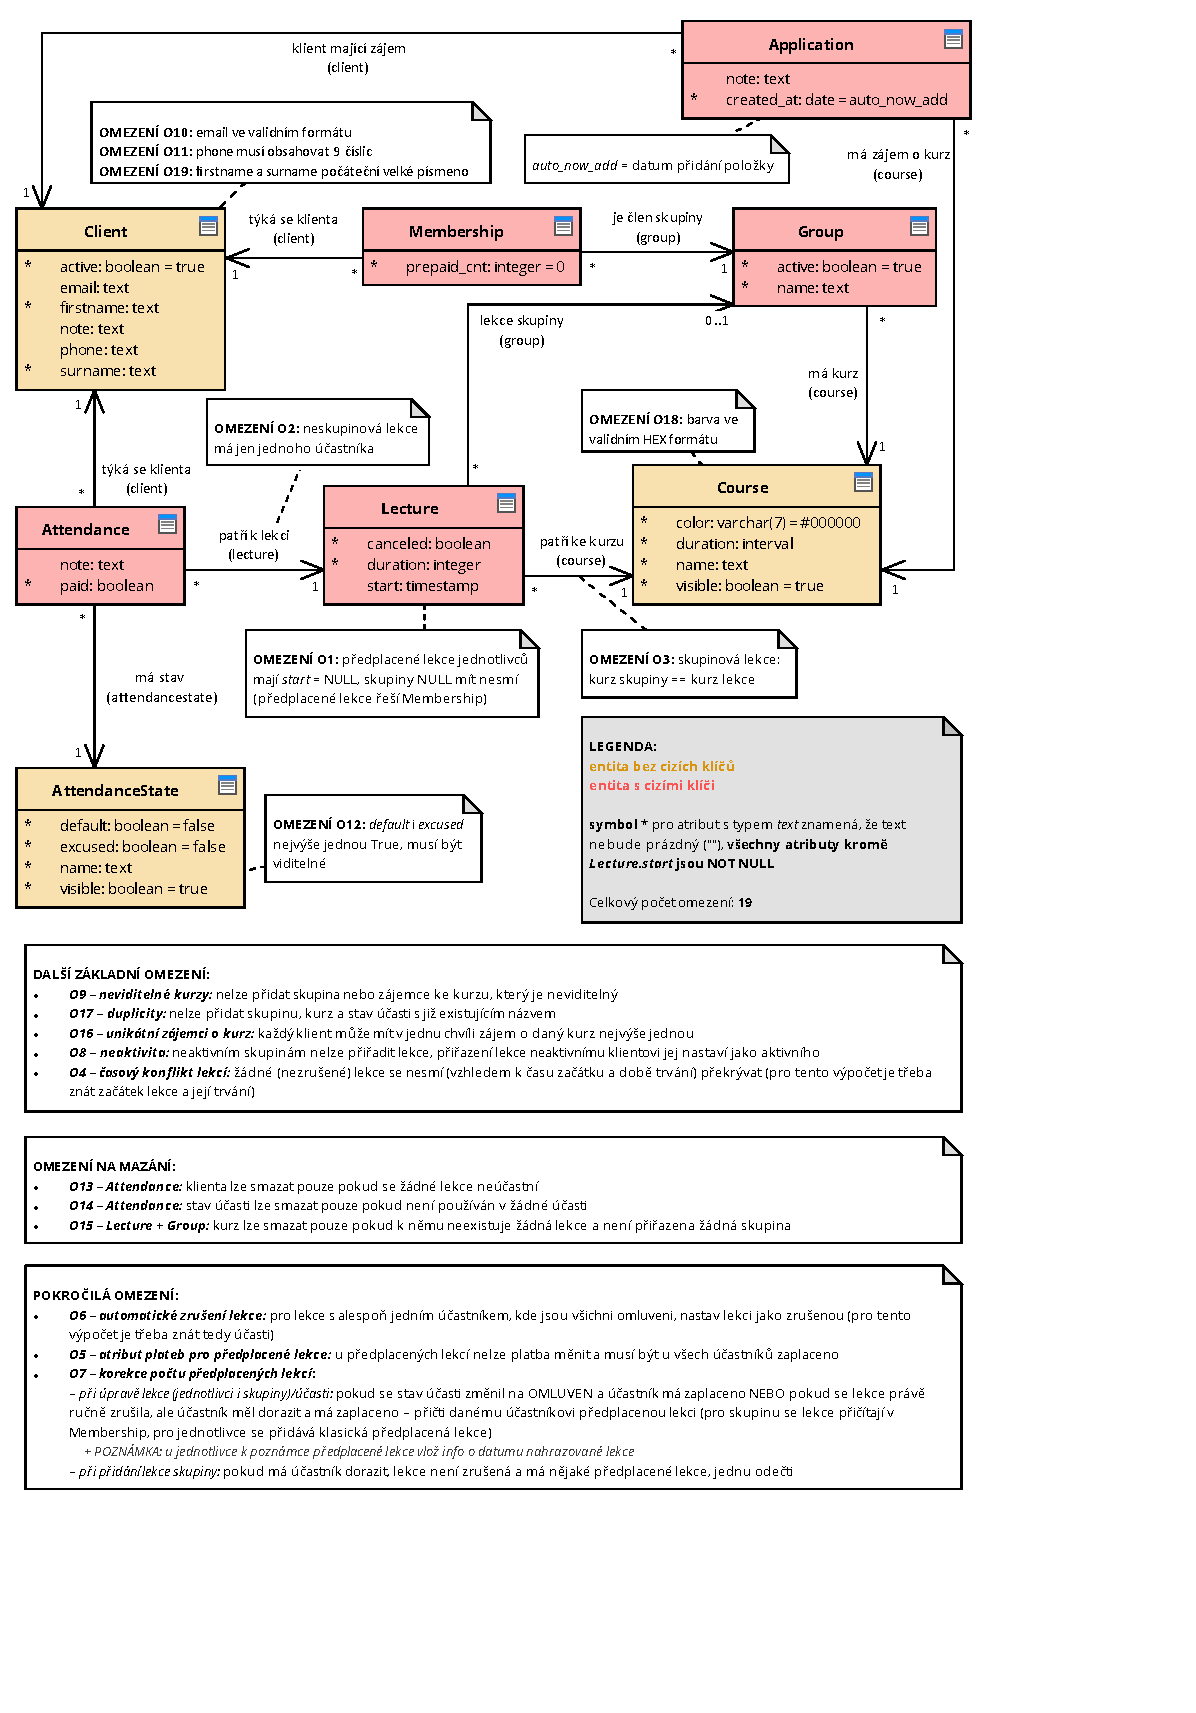
\includegraphics[width=1\textwidth]{img/db-model}
	\caption[Aktualizovaný logický datový model]{Aktualizovaný logický datový model}\label{fig:db-model}
\vspace{-15pt}
\end{figure}

\section{Komunikační rozhraní}

Ukázalo se, že původní komunikační rozhraní (REST API) z bakalářské práce mělo velmi dobrý návrh, bylo třeba provést pouze drobnější úpravy a především začlenit všechny potřebné změny z požadavků a datového modelu. Nejprve se zaměřím na drobnější změny a poté na začlenění změn z požadavků a datového modelu.

\subsection{Opravy a úpravy stávajícího rozhraní}

Pro odpověď na GET požadavek na lekce (GET \verb|lectures/|) byl u každé účasti klienta klíč \verb|count| pro označení pořadového čísla lekce. Zde jsou dva problémy. Prvním je fakt, že název klíče není úplně přesně vypovídající název vzhledem k dané situaci a při práci v kódu nastávaly nedorozumění, proto došlo k přejmenování na \verb|number|, což lépe odpovídá tomu, že se jedná a pořadové číslo lekce. Druhý problém je, že se z neznámého důvodu tento klíč vyskytoval u každé účasti v rámci lekce, což v případě lekce jednotlivce není důležité, ale v případě skupiny je pak totéž číslo u každé účasti (protože se řeší celkový počet lekcí, nikoliv zda konkrétní klient na nějaké lekci byl) -- tedy zbytečně se informace duplikuje a na klientské části se vezme její první výskyt -- toto bylo opraveno a pořadové číslo lekce se nyní vyskytuje přímo u lekce, nikoliv u každé účasti.

Součástí odpovědi GET \verb|lectures/|, jak již bylo zmíněno, je také přehled účastí jednotlivých klientů, zde bylo rozhodnuto také o odstranění vnořených informací o stavech účasti jednotlivých klientů -- v praxi zde byl poslán vždy název účasti, ID (a nově vzhledem k novému datovému modelu by byly poslány i informace \verb|default| a \verb|excused|), vzhledem k plánovaným změnám v rámci požadavku~\ref{N6} tyto vnořené informace byly odstraněny a nahrazeny pouze ID stavu účasti, protože si klientská část aplikace bude stavy účasti pamatovat (implementace viz TODO).


\subsection{Rozšíření rozhraní}

Rozhraní je třeba rozšířit o nové požadavky a úpravy datového modelu. 
+ pocty lekci a dalsi, filtry??

TODO - atributy z modelu

TODO - entity z modelu

TODO - banka

\section{Architektura}
    
\begin{figure}\centering
	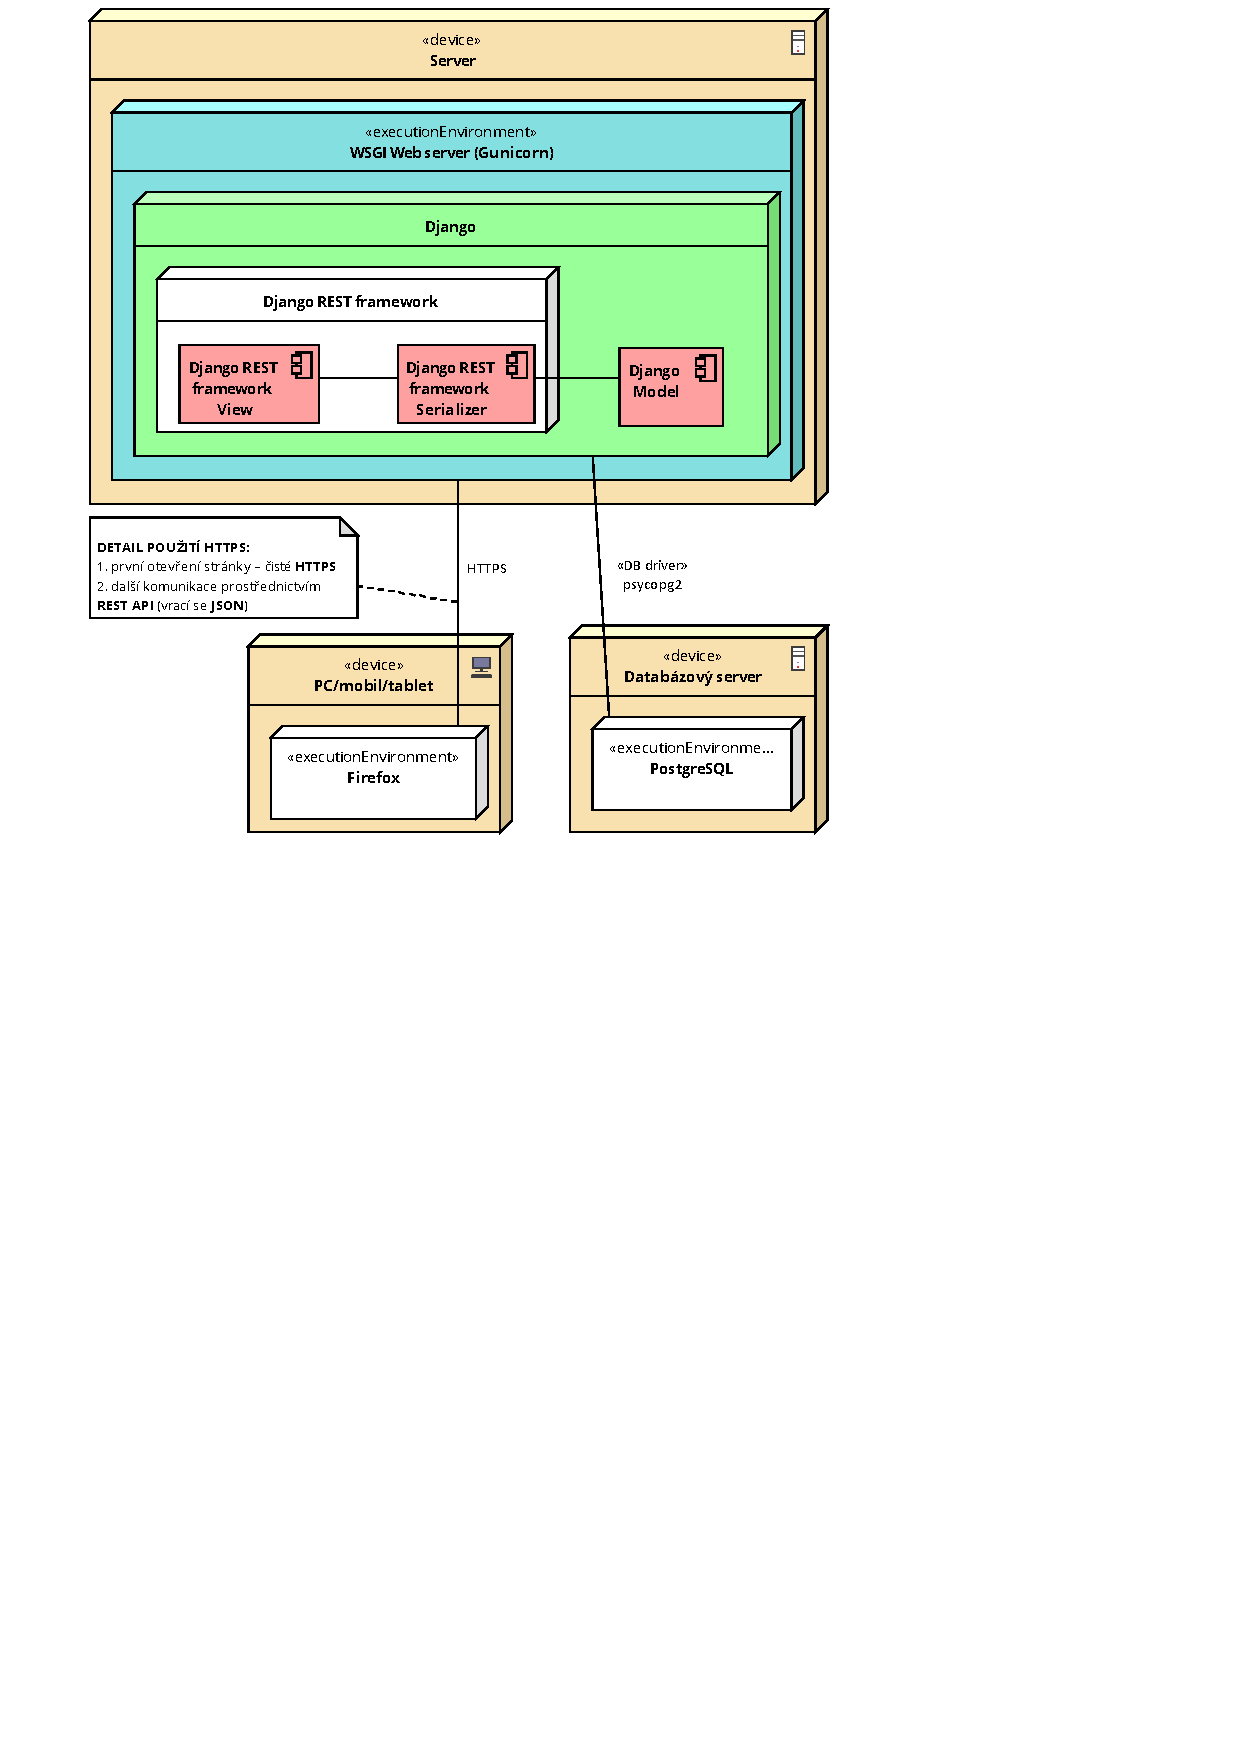
\includegraphics[width=1\textwidth]{img/deployment-diagram}
	\caption[Diagram nasazení]{Diagram nasazení}\label{fig:deployment-diagram}
\end{figure}

Aktualizovaný diagram nasazení na obrázku~\ref{fig:deployment-diagram} vychází z původního diagramu \cite{bp}. Jádro zůstává stejné a kromě drobnějších vylepšení pro zlepšení přehlednosti je v něm pouze jedna důležitá změna. V původním diagramu byl jako protokol pro komunikaci mezi serverem a klientem uvedeno HTTP/S. Vzhledem k požadavku na revizi bezpečnosti~\ref{N4} a jeho následné detailní analýze~\ref{subsec:N4detail} je v problému~\ref{B4} zmíněno zavedení HSTS. Podrobnému popisu se budu věnovat v TODO, důležitý je ale dopad na návrh architektury, kde díky zavedení HSTS a korektní konfiguraci aplikace všechna komunikace bude probíhat z důvodu bezpečnosti pouze přes HTTPS (Hypertext Transfer Protocol Secure).

\section{Konfigurace více prostředí}\label{sec:konfiguraceviceprostredi}

TODO

\section{Uživatelské prostředí}

Do klientské části bylo třeba navrhnout několik prvků z požadavků. Drobnější změny zde ukázány nebudou, zaměřím se jen na nejdůležitější změny v uživatelském rozhraní. Návrhy obvykle probíhaly na papír, ale pro lepší čitelnost je zde uvádím překreslené v aplikaci \href{https://pencil.evolus.vn/}{Pencil}.

\begin{figure}[h]\centering
    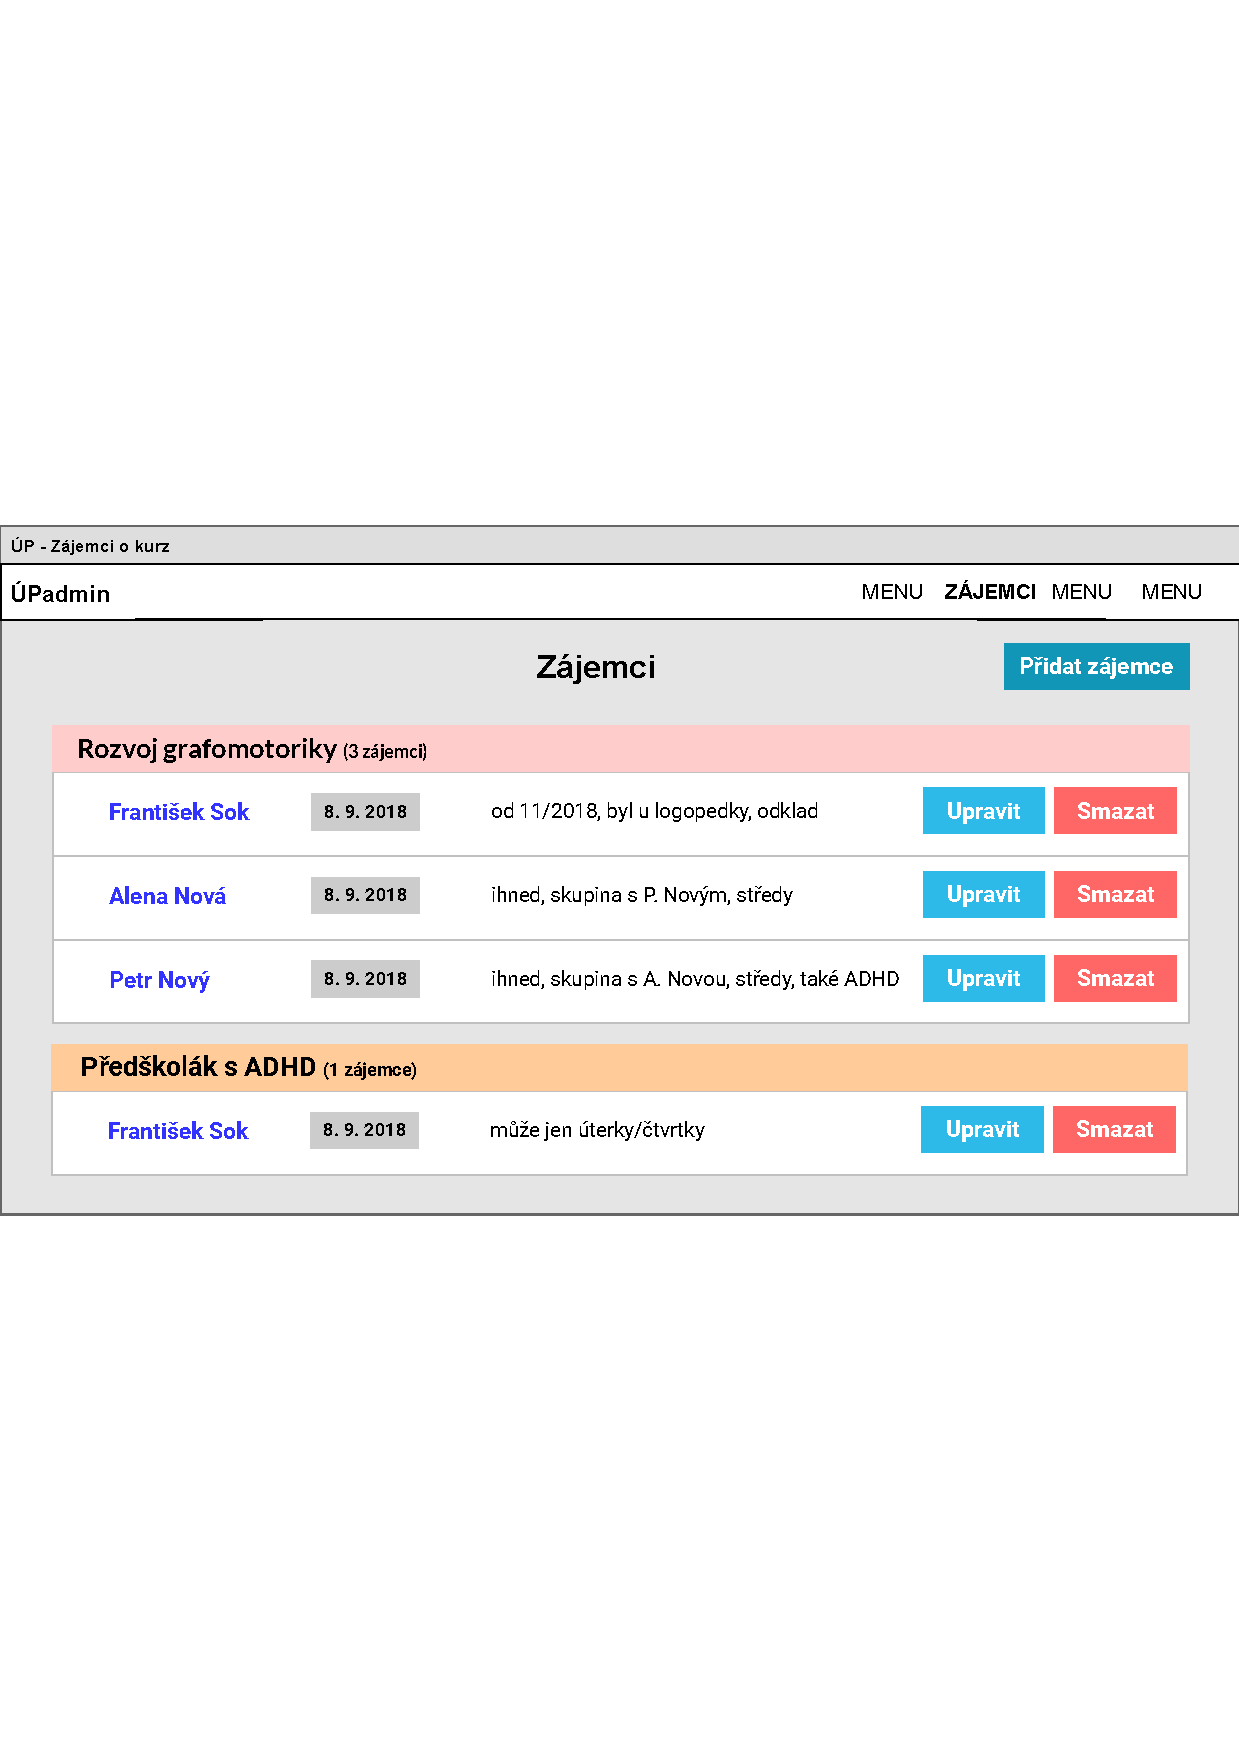
\includegraphics[width=1\textwidth]{img/ui-zajemci}
    \caption{Návrh zájemců o kurzy}\label{fig:ui-zajemci}
\end{figure}

Nejvýraznější změnou v klientské části je přidání nové stránky se zájemci kurzu (viz požadavek~\ref{F1}). Návrh je na obrázku~\ref{fig:ui-zajemci}, jak lze vidět, jsou barevně odlišeny kurzy -- zde již počítám se zavedením požadavku~\ref{F12} pro evidování barev kurzů (změny budou v implementaci učiněny napříč celou aplikací). Návrh splňuje všechny požadavky lektorky, kromě jednoduše dostupné úpravy je také dostupné tlačítko pro smazání -- to je obvykle napříč aplikací dostupné až v modálním okně s úpravou (protože se obvykle stejně nepoužívá a díky tomu, že není přímo na příslušné hlavní stránce, nemůže být ani omylem stisknuto a potvrzeno smazání ve vyskakovacím okně), zde je přímo u každého zájemce, protože oproti ostatním případům zde frekvence mazání bude vysoká vzhledem k postupnému obsluhování všech zájmů o kurzy.

\begin{figure}\centering
    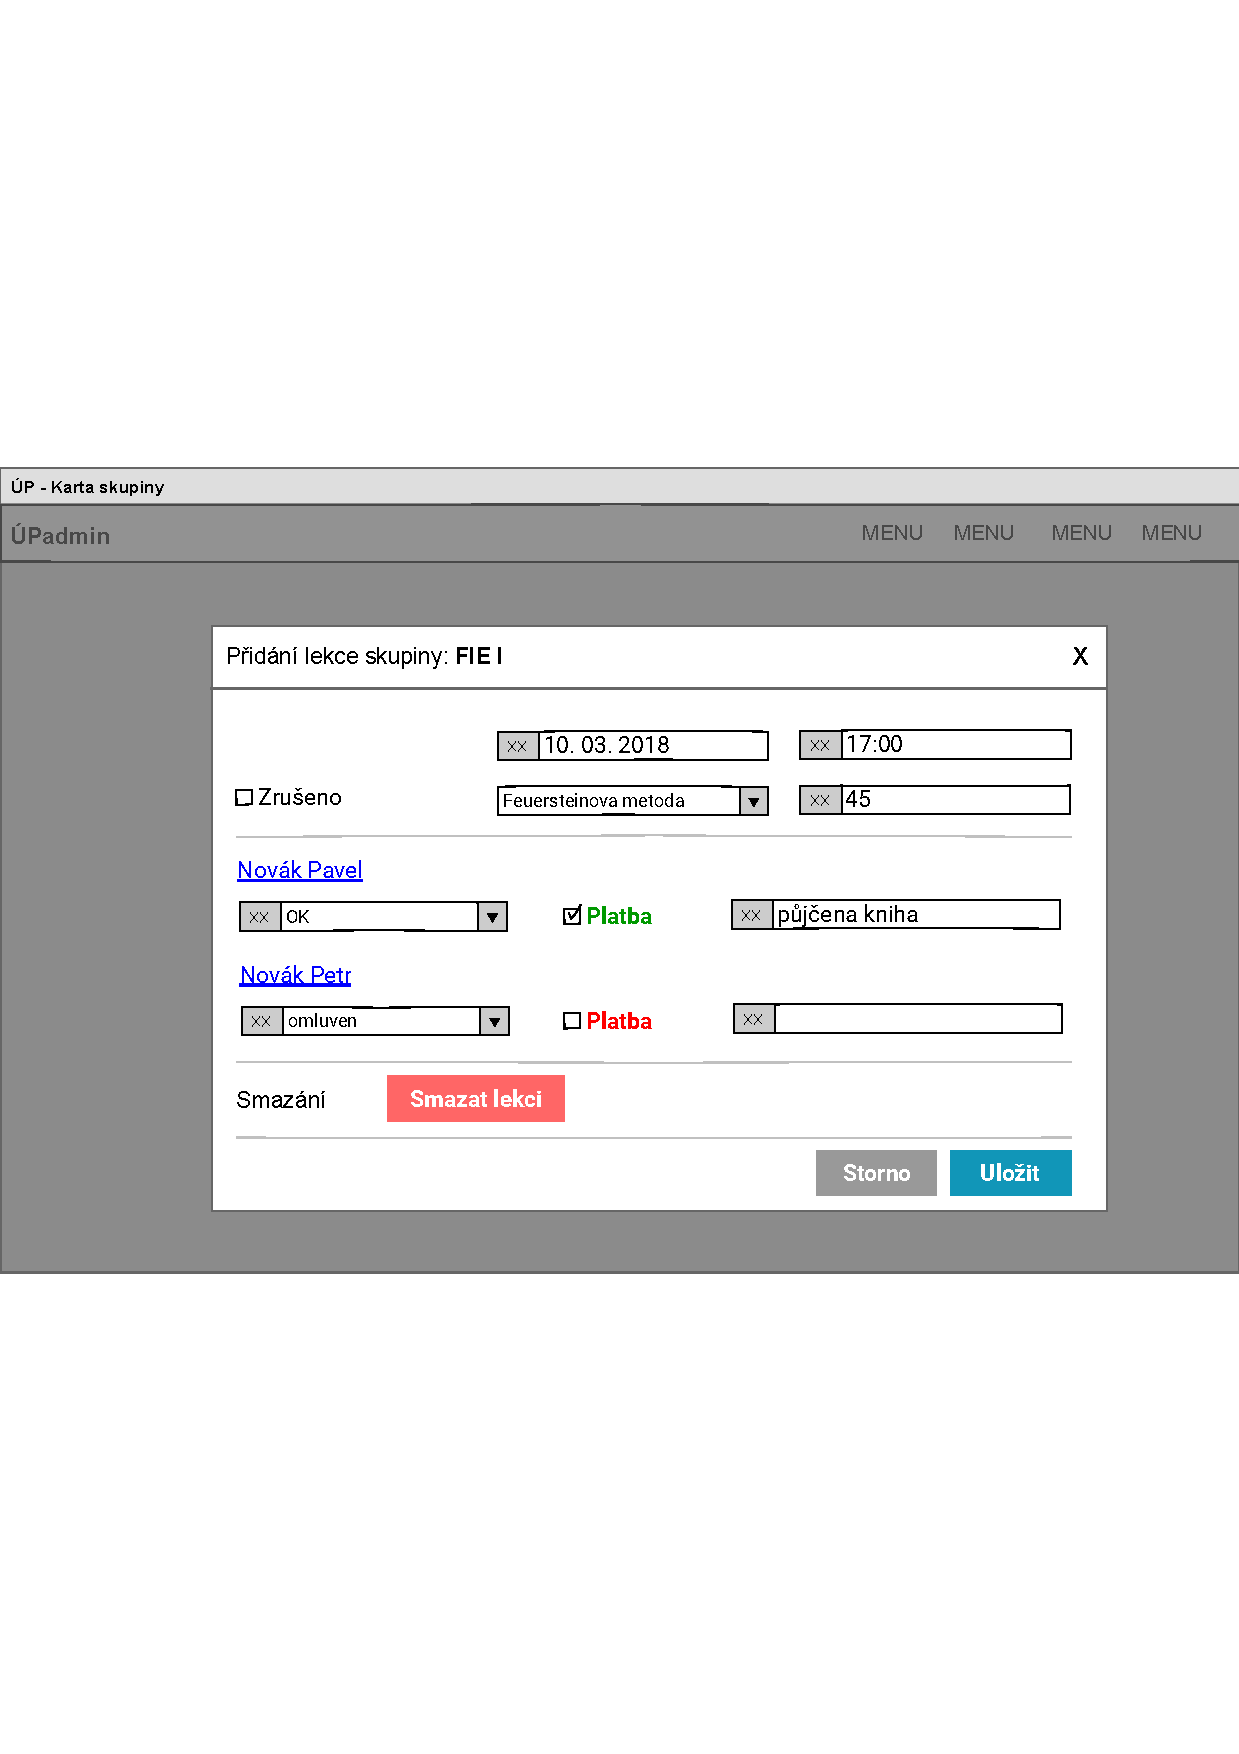
\includegraphics[width=1\textwidth]{img/ui-lekce-skupina}
    \caption{Návrh nového formuláře pro skupinové lekce}\label{fig:ui-lekce-skupina}
\end{figure}

\begin{figure}\centering
    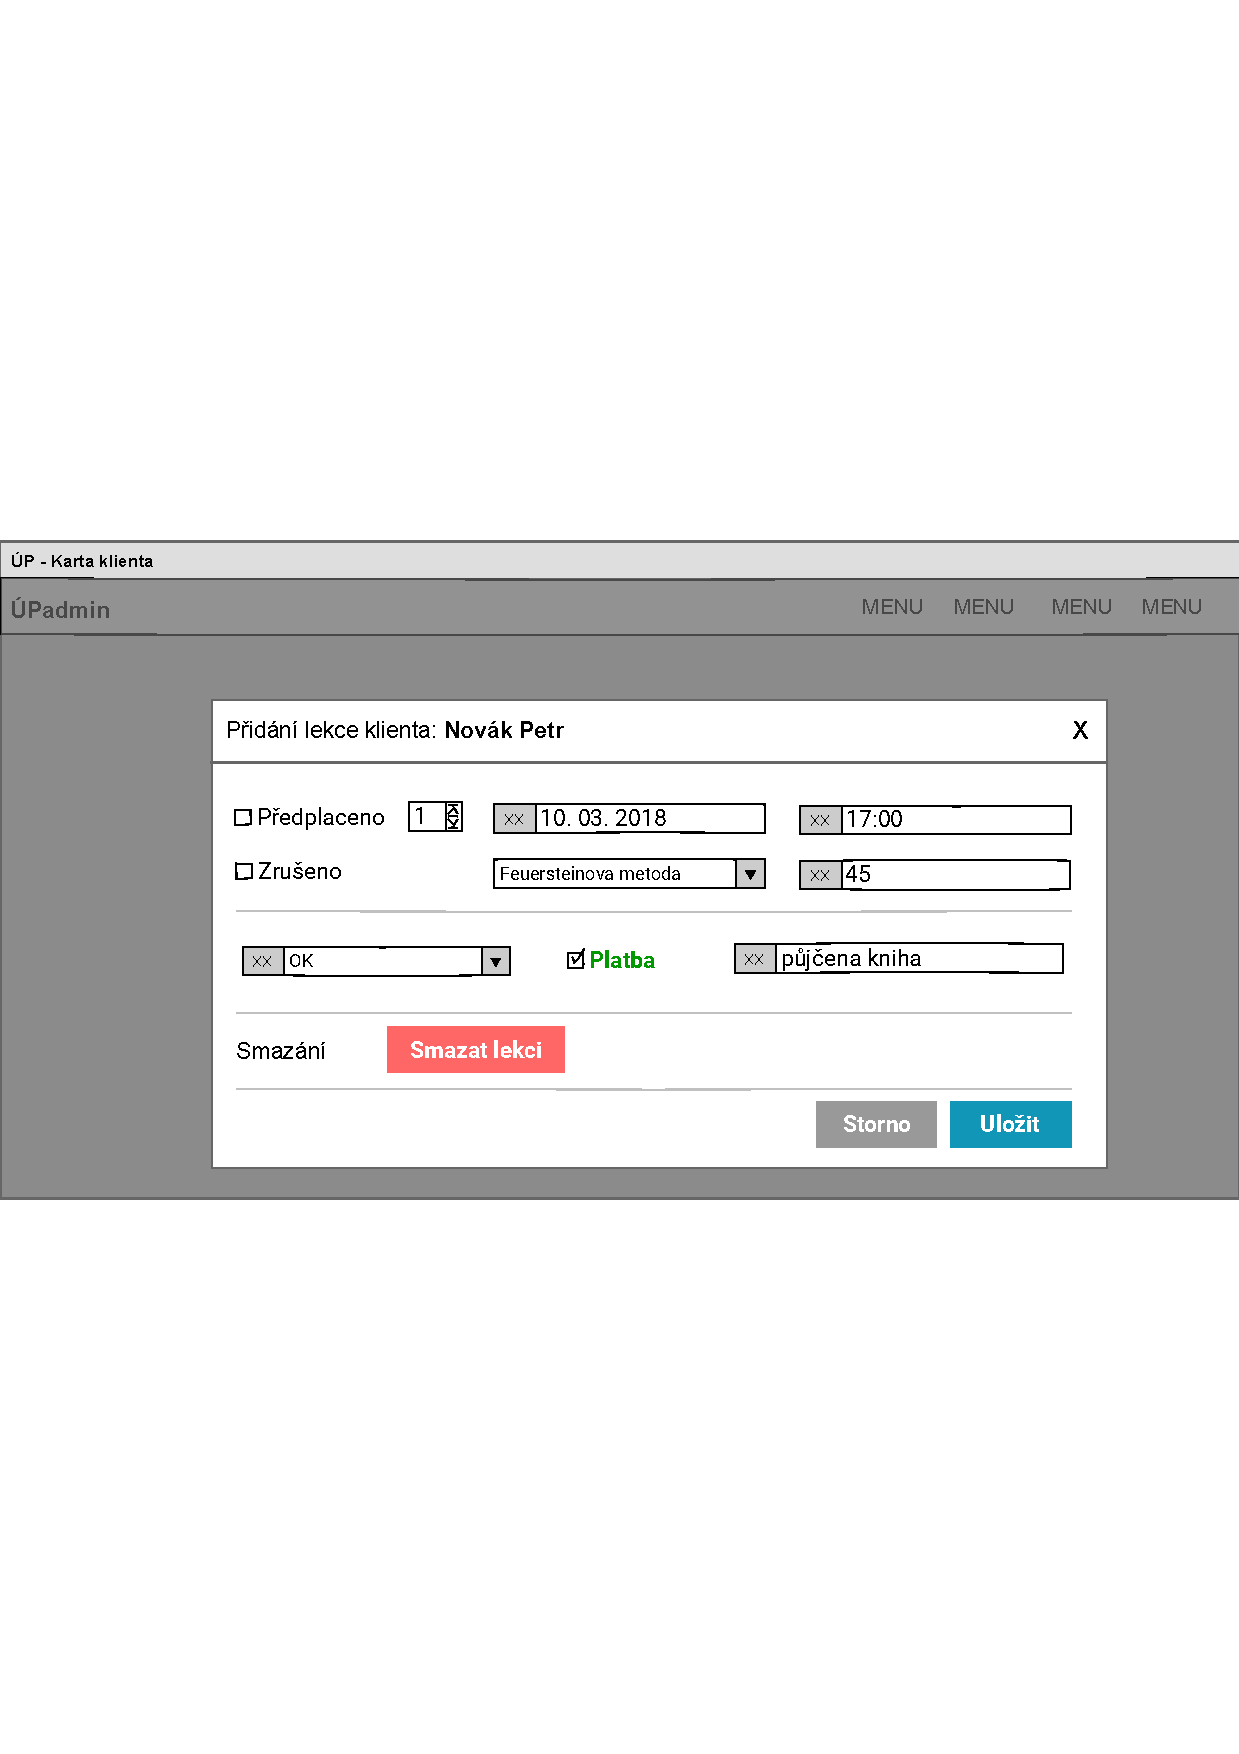
\includegraphics[width=1\textwidth]{img/ui-lekce-klient}
    \caption{Návrh nového formuláře pro lekce jednotlivců}\label{fig:ui-lekce-klient}
\end{figure}

Na obrázcích~\ref{fig:ui-lekce-skupina} a \ref{fig:ui-lekce-klient} jsou kompletně přepracované návrhy formulářů pro přidání (a potažmo i úpravu) lekce skupiny, resp. klienta. V rámci příslušného požadavku~\ref{F5} bylo třeba postupnými iteracemi dojít k návrhu, který umožní jednoduší práci s tímto formulářem, který je nejpoužívanější v rámci celé aplikace. V rámci detailní analýzy požadavku~\ref{F3} bylo zjištěno, že je třeba usnadnit přidávání více předplacených lekcí pro jednotlivce, tento požadavek v rámci tohoto přepracování formuláře pro lekce byl též začleněn -- pro klienty je v levém horním rohu dostupné pole pro zapsání počtu předplacených lekcí. Toto pole bude možné upravit při zaškrtnutí volby \enquote{Předplaceno}. Znaky \enquote{XX} u polí naznačují přítomnost ikony vysvětlující význam příslušného pole (místo textů, alternativní text se samozřejmě zobrazí po najetí na ikonu).

\begin{figure}\centering
    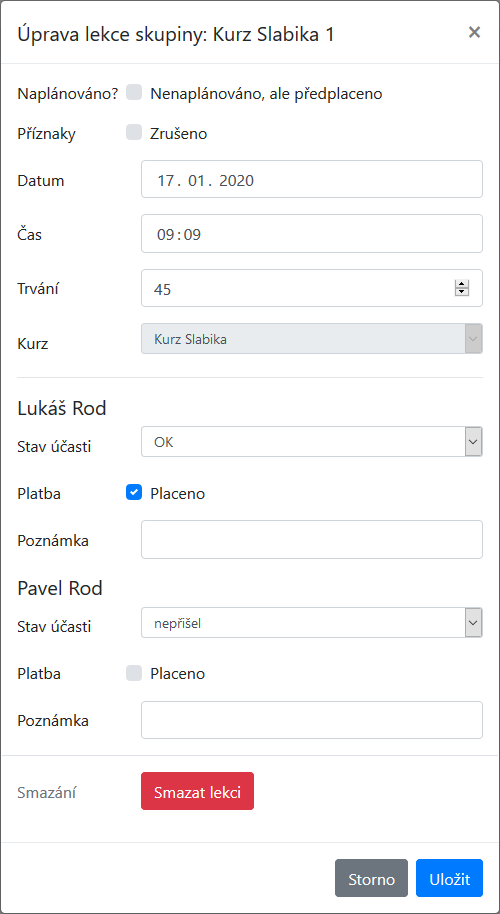
\includegraphics[width=0.52\textwidth]{img/ui-screen-lekce-skupina.png}
    \caption{Původní formulář pro lekce skupin}\label{fig:ui-screen-lekce-skupina}
\end{figure}

Díky větší šířce formuláře bylo možné vměstnat více polí na méně řádků, díky tomu a také ikonám došlo k ušetření místa, díky nově zobrazeným účastem klientů též ve formě řádků, navíc s odlišenou barvou platby je umožněna přehlednější a jednoduší evidence. Jak bylo uvedeno v požadavku~\ref{F5}, jedním z hlavních problémů bylo, že ve skupině může být např. 6 dětí a formulář má pak výšku několika obrazovek a je prakticky nepoužitelný -- zjednodušený názorný příklad původního formuláře (pouze se dvěma účastníky pro jednoduchost, ale účastníků je obvykle mnohem více) je na obrázku~\ref{fig:ui-screen-lekce-skupina}. Formuláře pro skupiny a jednotlivce (klienty) se liší jak počítadlem pro předplacené lekce (u skupin tato možnost není, protože bude řešena počítadly v rámci karty skupiny, viz požadavek~\ref{F3}). Druhou odlišností je pak zobrazení jména účastníka, které v případě jednotlivce je samozřejmě zbytečné (je v horní části formuláře), v případě skupin je toto jméno klienta současně odkazem do jeho karty pro rychlý přechod v případě potřeby.

\chapter{Implementace}
součástí sekce bude i sypani popela na hlavu za chyby v bakalarce - popisu co vsechno se delo, co bylo za problemy (napr bad patterny v reactu, coz zpusobilo ruzne problemy)

% todo migrace na novy react

PR:
* chyby při práci s modálními okny https://github.com/rodlukas/UP-admin/issues/95 - issue reactstrapu, vyjde nova verze
* react fontawesome PR pro vylepseni typescript podpory (ID atribut..)
* reactstrap tooltip ios fix

\section{Implementace požadavků}
IMPLEMENTACE POZADAVKU z analyzy vyse

F15:
* frontend odolny proti padu diky ErrorBoundary
* drf zpracovavat ProtectedError https://github.com/rodlukas/UP-admin/issues/70
* podrobnejsi chyby z api
* osetreni v api (IO...)
* notifikace neprekryvaji menu
* osetreni vstupu (vcetne konecne plne funkcniho API)
* js vylepseni notifikaci - notifikace doplnene o nadpis a ikonu, sjednoceny font, komponenta pro obsah notifikace, delsi doba zobrazeni error notifikace
* podrobnější chybové hlášky (např. při ProtectedError, když se uživatel pokouší mazat instanci, na které závisí jiné instance s chráněným příslušným FK; podrobnější info o časovém konfliktu...)

F18:
* pokročilá validace duplicit apod.
* zruseni noveho omezeni "neaktivní klienty nelze přiřadit do skupin (UI je ani nezobrazí ve výběru)" - neaktivní klienti již mohou být členové skupiny
* velka pocatecni pismena jmena klienta i pro api, presun transformaci field z modelu do serializeru
* viz EA docs
* js zvyrazneni neaktivity skupin a klientu napric aplikaci https://github.com/rodlukas/UP-admin/issues/85

N3:
* refaktoring
* js komponenta pro zobrazeni lekci https://github.com/rodlukas/UP-admin/issues/71
* template strings js
* python refaktoring https://github.com/rodlukas/UP-admin/issues/93
* zavedeni prvnich hooku, drobna vylepseni komponent - prechod na funkcionalni komponenty, upravy komponent (napr. zbytecne pouzivaly stav nebo se zbytecne casto updatovaly, ikdyz to nebylo potreba) + **odstranění zbytečného stavu odstranilo i chybu, která byla už od počátku v aplikaci a způsobovala občasné nefungování komponenty s aktuálním stavem účasti - zobrazil se jiný stav, než byl skutečný, v závislosti na pořadí obdržení odpovědí od serveru, to se začalo víc projevovat při nedávných změnách architektury reactu**
* opravy nekonzistentnich stavu
* analyza pruchodu aplikaci (google analytics)
* opravy nevalidniho html a css (diky tomu lepsi zarovnani tlacitek)
*  js useEffect - exhaustive deps https://github.com/rodlukas/UP-admin/issues/96
* prechod na TS: dalsi zmeny viz https://github.com/rodlukas/UP-admin/releases/tag/1.0.0
* Minifikace HTML
* oprava práce se setState - zbytečně se přes const state = this.state nastavoval pak ve setState celý nový stav, což je zbytečné a navíc to může způsobovat problémy při dalším volání setState (které když proběhne před tímto, může přijít v niveč, protože jej nahradí tato kompletní změna stavu, ačkoliv se má měnit jen malá část stavu komponenty) 

F8:
* zobrazují se transakce za posledních 14 dnů, FIO omezuje dotazy na API na 30 s, takže server cachuje odpověď banky rovnou 60 s, zobrazuje se i aktuální zůstatek + barva je podle toho, zda je na účtu dostatek peněz na zaplacení nájmu (zelená, resp. červená s upozorňujícím vykřičníkem s dalšími informacemi), po 60 s možnost výpis obnovit, případně lze jít do bankovnictví, opravuje \#50
* cache, upozorneni na najem

* "noopener noreferrer" z důvodu bezpečnosti
* robots.txt, pak nahrazeni robots.txt meta tagem pro uplny zakaz cehokoliv robotum
* pipfile
* mnoho promennych prostredi → ve všech prostředích se pracuje stejným způsobem s příslušnými proměnnými prostředí, je čistější nastavení Djanga a umožňuje díky .env souboru (je v .gitignore) použít i lokální proměnné prostředí (jinak těžko univerzálně nastavitelné i v rámci IDE) + odstranění zašifrovaných proměnných v konfiguráku travisu a přesun přímo do repo
* zobrazení tel. čísel klientů v zájemcích o kurz (\#61)
* oprava logiky výpočtu "příště platit" - nebral v úvahu předplacené lekce (https://github.com/rodlukas/UP-admin/commit/e84aa4eec9bb93323a097830dd1416204658c87a)
* lekce je automaticky zrušená na frontendu i backendu když jsou všichni účastníci omluveni, na to je příslušně uživatel upozorněn ve formuláři (a zároveň zrušení nejde měnit, protože by backend lekci stejně tak či tak zrušil)
* rozdělení CSS stylů ke komponentám
* asynchronní update všech dní v týdnu v diáři při nějaké změně (ca53c16), opravuje \#19
* zjednodušení kódů a struktury souborů, refactoring, odstranění všech zbytečných getDerivedStateFromProps (nahrazeno např. componentDidUpdate)
* migrace na nový životní cyklus komponent Reactu (503b9ac)
* funkční zobrazení vývojové verze na jiném zařízení v síti
* oprava chyby způsobující nekorektní zobrazení lekcí v předchozím dnu - když např. byla lekce v 1 h ráno, v diáři se ukázala v předchozím dni jako poslední → porovnávávání datumu s TZ s datumem bez TZ → vyřešeno použitím "\_\_date" v querysetu (3da9db1)
* oprava chybné práce s datumem v diáři (JS) - pokud se zadala URL s datumem, kde den měl číslo "31", došlo k "přesunu do minulosti" (číslo dne se změnilo na "1") - v důsledku toho se v aplikaci nedalo dostat do roku 2019, protože 31.12.2018 bylo pondělí a další týden se přepnul na listopad
* 05-2019 prechod na nwb
* mene pozadavku - react context api (attendancestates + nově také viditelné kurzy, aktivní klienti/skupiny - vše napříč aplikací) -> TÍM PÁDEM POTŘEBA PŘEJÍT NA NOVÝ REACT -> je tedy potřeba provést i migraci na nový lifecycle reactu, vice viz https://github.com/rodlukas/UP-admin/releases/tag/0.8
* redesign vsech stranek pro lepsi konzistenci, srozumitelnost a pochopeni (predelany diar, zajemci, lekce v karte...)
* Pro zrychlení načítání celé aplikace se používá lazy loading React.lazy + React Suspense - umozni kratsi prvni nacteni appky, zalozene na react-routeru + reseni nastaleho problemu -- reseni Error: Loading chunk 11 failed. https://github.com/rodlukas/UP-admin/issues/92
* optimalizace frontendu - odstraneni komponent definovanych primo v render - mohlo zpusobit potize s vykonem i nechtenym prekreslovanim vnorenych komponent
* úprava stavových kódu API pro bankovnictví (\#55) - už vrací jen 200/500, ostatní chyby jsou zahrnuty v 500 a podrobnější informace jsou přiloženy do JSONu rovnou na serveru (tedy na frontendu není žádná logika navíc)
* úpravy a opravy API - na backendu nechybí žádná logika, která doteď mohla být třeba i jen na frontendu - už fungují všude PATCH metody, kód API je rozumnější, efektivnější a přehlednější a nedělají se v něm zbytečné kraviny navíc, rozumně se např. už pracuje i s takovými atributy, které lze zaslat na API jako null, ošetření všech možných případů - opravuje \#52

    kompletní validace tel. čísla na backendu i frontendu, vylepšení způsobu validace a dělení čísla na mezery už při psaní o formuláře, následné odstranění mezer až na backendu
    oprava chyby způsobující chybu při úpravě stavu účasti předplacené lekce
* odstranění křížku pro reset react-selectu, aby nedocházelo k vymazání "omylem", když funkcionalita stejně není třeba
* občas se využívají skupinové lekce bez definovaných účastníků (ještě nejsou známí), taková lekce se ale ukazuje jako zrušená a u skupiny chybí info, že nejsou žádní účastníci - potřeba vylepšit zobrazení


N4:
* contextapi pro prihlasovani - zmeny viz https://github.com/rodlukas/UP-admin/releases/tag/0.8

N6:
* DRF-JWT problémy, dotazy na SQL DB ikdyž nemají být - https://github.com/rodlukas/UP-admin/issues/51 - přechod na jinou knihovnu a zde PR na překlad do CZ
* pomalé SQL dotazy- obri optimalizace dotazu na DB (>4x zrychleni) diky DJDT, pokrocile optimalizace
* odstraneni zbytecne prace s DB napric api - zrychleni - commit https://github.com/rodlukas/UP-admin/commit/ba12eea6be642d0c56629ac607fb1f8ffab267f7
* vice info viz https://github.com/rodlukas/UP-admin/releases/tag/0.9.0

F6: 
* pri uprave/pridani skupiny/klienta dojde automaticky k prepnuti na zalozku aktivni/neaktivni podle toho, do ceho jsme pridavali

\section{Zavedení nástrojů pro usnadnění vývoje a údržby}
podrobny popis jak probihalo zavedeni, co mi to umoznuje, treba i screenshoty, k cemu to bylo pouzito, jak se to osvedcilo - nastroje vychazi ze zvolenych nastroju z reserse


LGTM: 
[js] odstraneni unused promenne v Applications
[js] oprava spatneho nazvu promenne v inicializaci ErrorBoundary
[js] oprava potencialnich chyb zpusobenych nespravnou aktualizaci stavu
[python] odstraneni vsech import *
[python] optimalizace importu
[js] optimalizace importu
[js] oprava primeho zapisovani do stavu v Card
[js] konzistentni stav PrepaidCounters
[js] konzistentni stav at\_state ve FormLecture

sonarcloud viz commity koment


sider PR
houndCI PR
codefactor nefunkcni dependence stylelint, eslint config js nepodporuje
code-inspector - katastrofalni UI, naprosto nefunkcni parsovani, importy nefunguji... (v UI nefunguje ani tlacitko zpet a vse je rozpadle...)


deepcode
deepscan, sonarcloud, lgtm
deepsource
codebeat
codeclimate
codacy
 
\begin{itemize}
\item ...
\item code formatting - prettier, black
\item python zavedeni vulture pro dead code
\item napojeni na Sentry, Slack, logentries, GA
\item zavedeni LGTM, opravy nalezenych problemu
\item travis: zavedeni cache pro yarn a pipenv, zjednoduseni prace s .npmrc, na heroku se neprovadi build a collectstatic
\item zmena react toolkitu (nejdrive nwb, pak test neutrinojs a nakonec custom webpack + porovnani size bundle), viz https://github.com/rodlukas/UP-admin/issues/67 a https://github.com/rodlukas/UP-admin/issues/65
\item ...
\end{itemize}


\chapter{Testování}
implementace samotneho testovani v behave, Selenium



N2: 
* vylepseni vsech testu - neprobihala kontrola zobrazenych dat ve formulari pred upravou
* zrychleni testu upravy klientu
* vylepseni potvrzovani formulare pro lepsi zachyceni chyb
* oprava náhodně občas nefungujících testů na CI (po každém scénáři je smazána localstorage) (\#64)

\begin{itemize}
\item popis, jak jsem konkretne tvoril vsechny UI/API testy v behave a seleniu, co bylo za problemy (nacitani, viz heuristika), jak to funguje, jak jsem vsechno udelal
\item coverage 86 \%
\item popsat co vsechno se testuje, ze je to v jazyku gherkin
\item popsat co se netestuje
\item pripadne zminit ze bylo reseno v ramci MI-PYT
\item popsat dalsi problemy s nehezkym API selenia, ktere je pro ruzne jazyky nejednoznacne a nesjednocene (mozna kvuli verzi 3, v4 uz asi bude lepsi...), hrozna dokumentace, ale zase to pouzivaj vsichni tak se vsechno vsude najde
\item pripadne dodat akceptacni testovani
\item niels. heur. analyza, ktera pomohla pak v implementaci prakticky zprovoznit UI testovani, protoze co nevi clovek, nevi ani selenium a tezko se neco testuje (nevi ze se nacita kdyz to nevidi ani clovek, nevi ze se ma cekat..)
\item mozna zminit usability testovani - zejmena proto, ze prakticky na tom stoji dalsi vylepseni v analyze, kde jsem pozoroval lektorku pri bezne praci a na zaklade toho jsme resili, co by chtela zmenit/pridat/upravit; tady neni treba testovat pro jine uzivatele, je to zamerene na interni pouziti 1 clovekem, o to lepsi to ale musi byt:)
\end{itemize}


\chapter{Nasazení}
popis toho jak jsem udelal novej zpusob nasazovani
* django-environ

\section{Zavedení více prostředí}
\begin{itemize}
\item vyvoj BP probihal na lokalu a pak probehl push na GH, travis provedl build a testy a nasadilo se na produkci, to znamená že jsem samozřejmě produkci mohl zbořit (a taky že párkrát zbořil..)
\item jak funguje stage, testing, produkce, demo co kam kdy jde v souvislosti s releasy, k cemu to je, jak se to osvedcilo - dohledavani problemu na stage kdyz se neco stane na produkci
\item (zustava dev a produkce)
\item pokročilé debugování na lokálním i vzdáleném prostředí díky Django Debug Toolbar 
\item vyhoda testing a demo env je ze tam muze kdokoliv, neuvidi nic duverneho (ani pristup do banky tu neni povolen), takze do toho muze vedouci prace, oponent i bezny uzivatel, da se testovat vse na obdobnem prostredi jako pak bude staging, produkce (heroku)
\item + samozrejme je zde moznost spustit na lokalu, ale todle je mnohem rychlejsi (viz GH)
\end{itemize}

\section{Další úpravy}
\begin{itemize}
\item automaticke zalohovani DB
\item ...
\end{itemize}



\chapter{Možná rozšíření}
klasika - co by se dalo delat dal, o co by se appka mohla rozsirit, dalsi technologie, fce

\chapter{Zveřejnění jako open-source}
repo na GH uz je pripravene: https://github.com/rodlukas/UP-admin - vcetne instrukci pro spusteni
\begin{itemize}
\item popsat proc zverejnit - moznost nahlednout na realnou aplikaci s nejnovejsimi technologiemi, jak je nakonfigurovana, inspirovat se + ma reference
\item MIT licence
\item popsat co bylo treba pro zverejneni udelat - priprava vsech casti, vyreseni tokenu, promennych prostredi... + problem: automaticky zverejneni buildu frontendu, aby ho clovek mohl pouzit pri spusteni u sebe na lokalu - protoze se pouziva placena knihovna, ke ktere mam pristup jen ja, takze si to nikdo jiny u sebe nezbuildi (resi to travis a nahraje build do assetu k release) - řešení: na travisu se provede build frontendu a ten se automaticky jako *zip* soubor nahraje k příslušnému github release 
\item na GH  je popsání vlastností, požadavků, postupu instalace a spuštění, testování + připravená vzorová data pro DB (včetně návodu na jejich vložení)
\item (? promenne prostredi mozna zminim i jinde)
\end{itemize}



